%%%%%%%%%%%%%%%%
\section{Inner Controller}

\begin{frame}{Inner Controller}{}
    \uncover<1-2>{
    \begin{figure}[H]
        \centering
        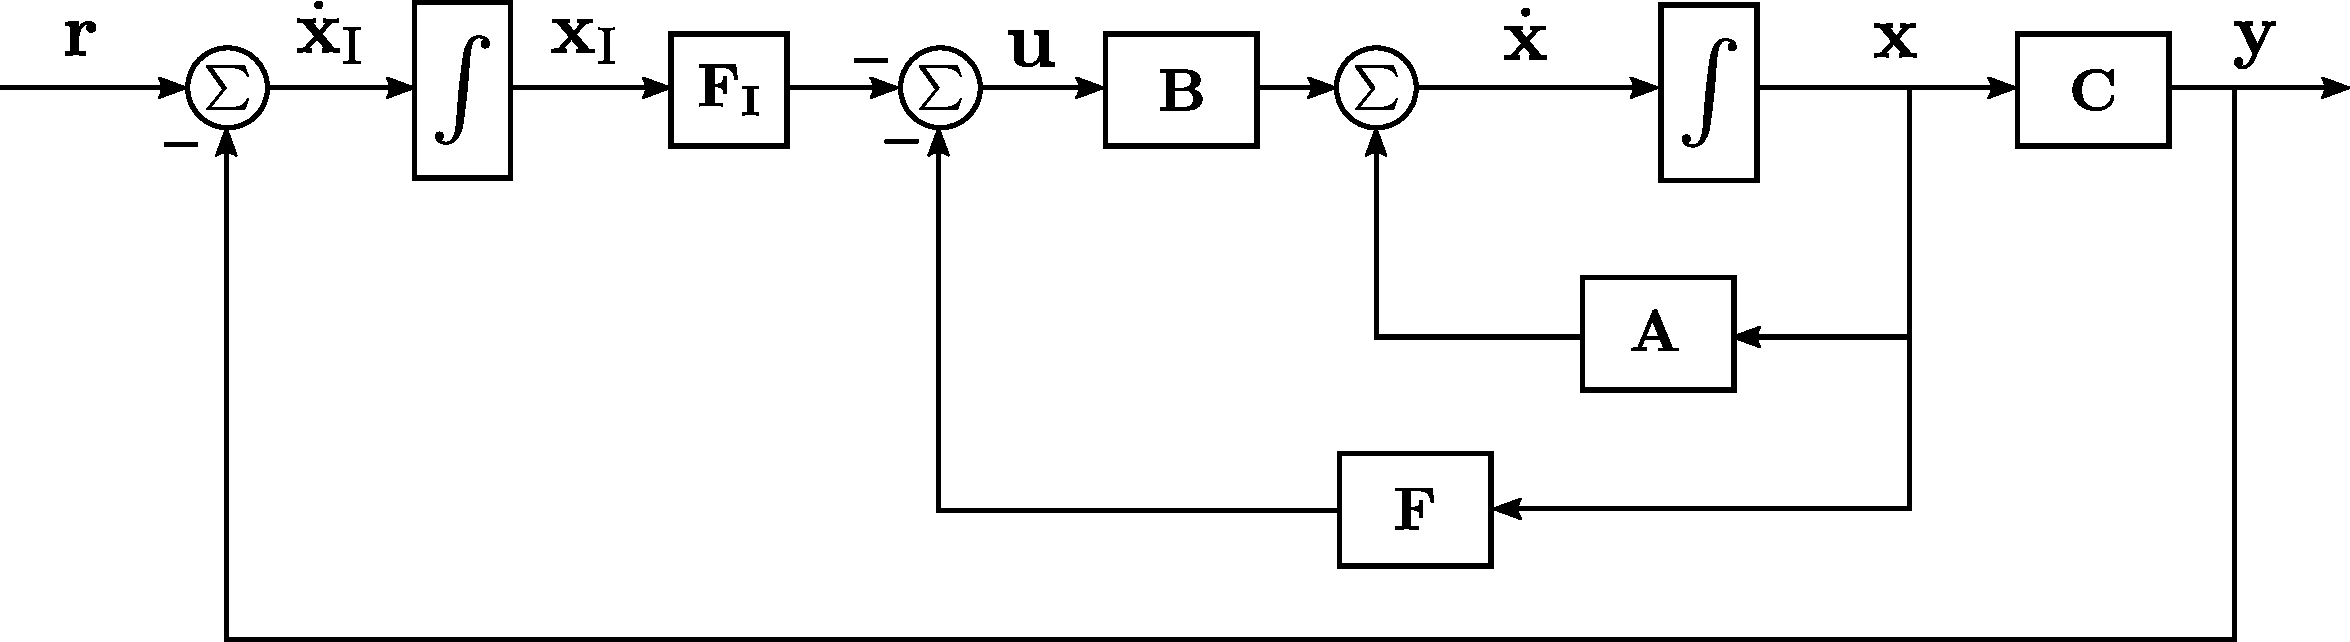
\includegraphics[width=1\linewidth]{figures/HinfControlBlockDiagram}
    \end{figure}}
    \uncover<2>{
    \begin{itemize}
        \item Linear Quadratic Regulator
        \item $\mathcal{H}_\infty$ Controller
    \end{itemize}}
\end{frame}

\begin{frame}{Inner Controller}{$\mathcal{H}_\infty$ Controller Design}
	%\begin{overprint}
	\uncover<1-6>{
	    \begin{figure}[H]
	        \centering
	        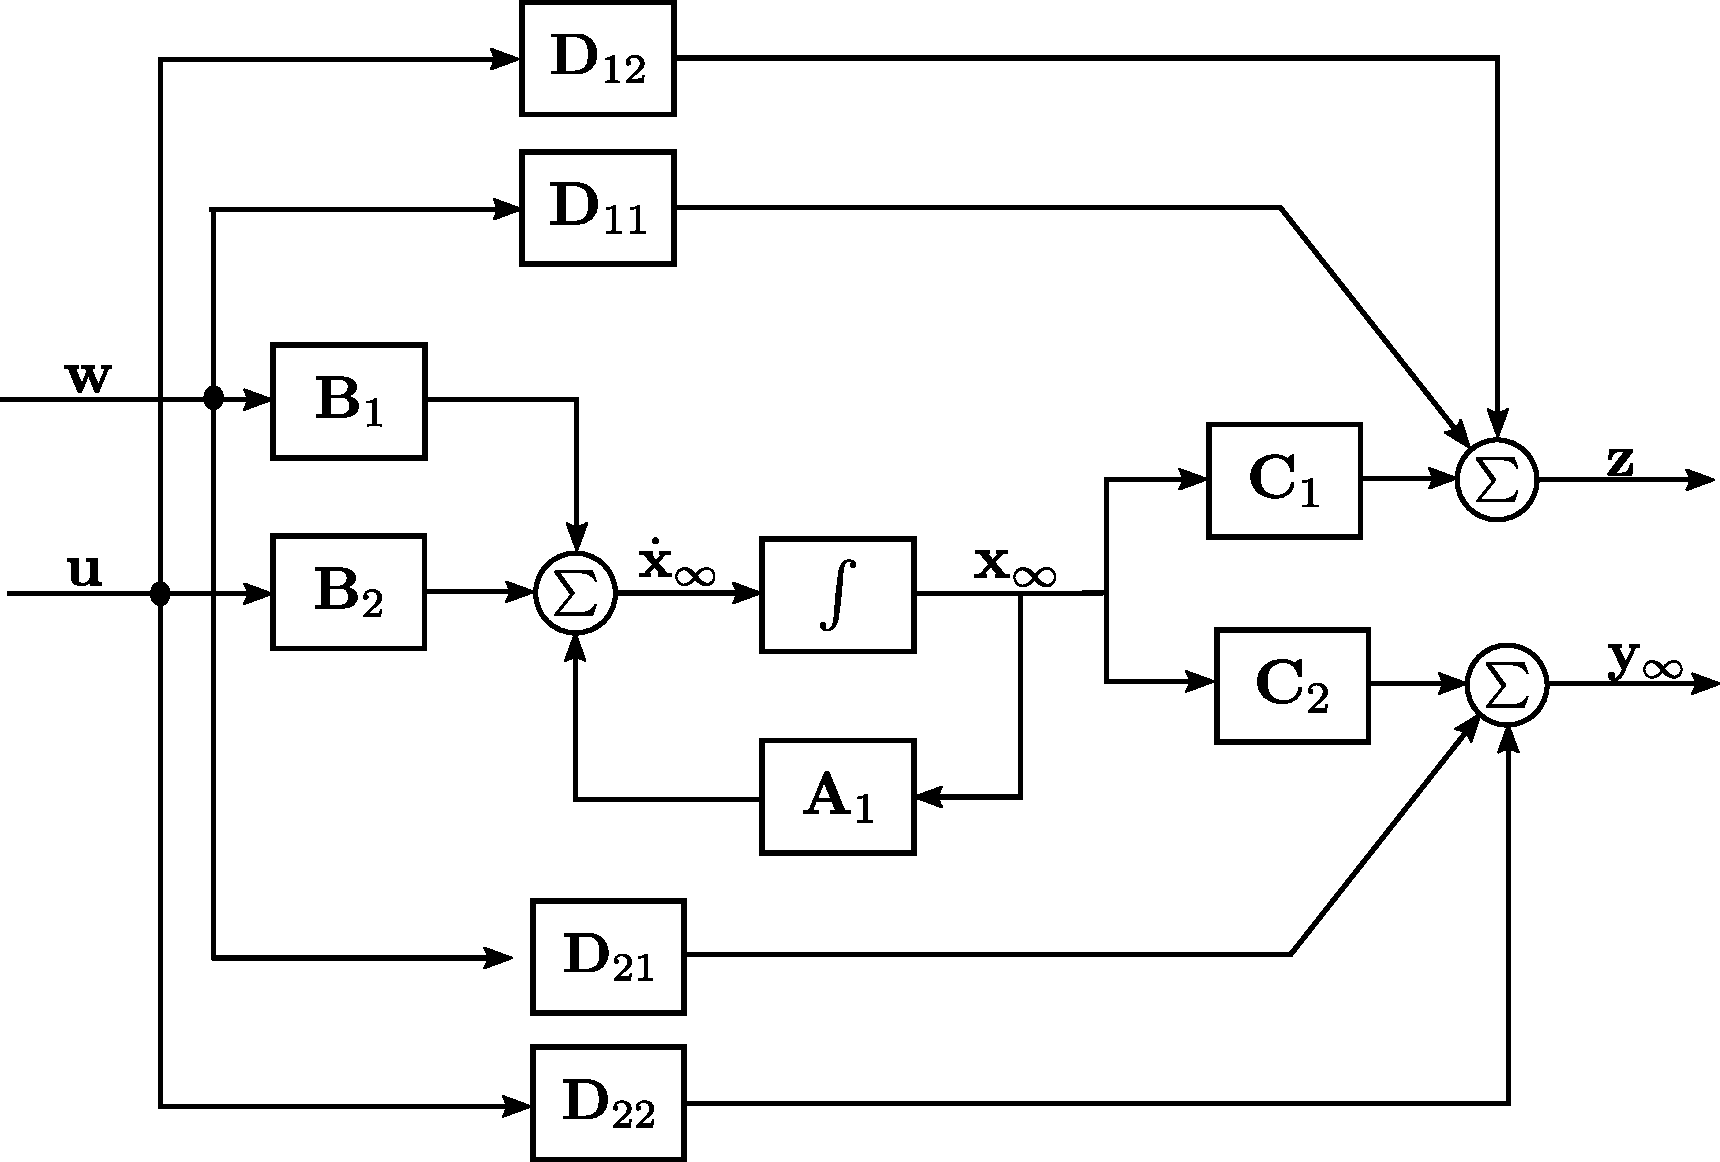
\includegraphics[width=0.6\linewidth]{figures/HinfDiag}
	    \end{figure}}
		\onslide<1>{
		\begin{flalign}
			\dot{\vec{x}}_\infty(t) &= \vec{A}_1 \vec{x}_\infty(t) + \vec{B}_1 \vec{w}(t) + \vec{B}_2 \vec{u}(t)\nonumber\\
			\vec{z}(t) &= \vec{C}_1 \vec{x}_\infty(t) + \vec{D}_{11} \vec{w}(t) + \vec{D}_{12} \vec{u}(t)\nonumber\\
			\vec{y}_\infty(t) &= \vec{C}_2 \vec{x}_\infty(t) + \vec{D}_{21} \vec{w}(t) + \vec{D}_{22} \vec{u}(t)\nonumber
		\end{flalign}}
		\onslide<2-6>{
		\begin{flalign}
			\vec{x}_\infty(t) &=
			\begin{bmatrix}
			\psi & \dot{\psi} & \dot{x}_\mathrm{b} & x_{int_{\psi}} & x_{int_{\dot{x}_\mathrm{b}}} & x_{F_\mathrm{wc}} & x_{\tau_\mathrm{wc}} & x_{F_\mathrm{wave}} & x_{\tau_\mathrm{wave}} & x_{n_{\psi}}\ \ \  x_{n_{\dot{x}_\mathrm{b}}}
			\end{bmatrix}^\mathrm{T} \nonumber 
		\end{flalign}}
%		\onslide<3>
%		\begin{flalign}	
%			\vec{u}(t) &= 
%			\begin{bmatrix}
%			F_1 & F_2 
%			\end{bmatrix}^\mathrm{T}\nonumber 
%		\end{flalign}
%		\onslide<4>
%		\begin{flalign}	
%			\vec{w}(t) &= 
%			\begin{bmatrix}
%			\psi_\mathrm{ref} & \dot{x}_\mathrm{b,ref} & F_\mathrm{wc} & \tau_\mathrm{wc} & F_\mathrm{wave} & \tau_\mathrm{wave}& n_{\psi} & n_{\dot{x}_\mathrm{b}}
%			\end{bmatrix}^\mathrm{T} \nonumber 
%		\end{flalign}
%		\onslide<5>
%		\begin{flalign}
%			\vec{y}_\infty(t) &= 
%			\begin{bmatrix}
%			\psi & \dot{x}_\mathrm{b} & \vec{x}_\mathrm{I}^\mathrm{T}
%			\end{bmatrix}^\mathrm{T}\nonumber 
%		\end{flalign}
%		\onslide<6>
%		\begin{flalign}	
%			\vec{z}(t) &= 
%			\begin{bmatrix}
%			\vec{x}_\infty^\mathrm{T} & \vec{u}^\mathrm{T}
%			\end{bmatrix}^\mathrm{T}\nonumber		
%		\end{flalign}
%	\end{overprint}
\end{frame}

\begin{frame}

\end{frame}

